\chapter{Fundamentação Teórica}
\label{c.fundamentacaoteorica}

Em Ciência da Computação, compressão de dados é o processo de codificar as mesmas informações usando um número menor de bits, sem que haja distorção dos dados originais. Em se tratando de compressão de imagens, pode-se alcançar Esse processo é útil, pois reduz o consumo de recursos computacionais, como espaço em disco, ou utilização de banda de internet.

Considere as imagens abaixo.

\begin{figure}[h]
\caption{\small Codificador e Decodificado de Imagens}
\centering
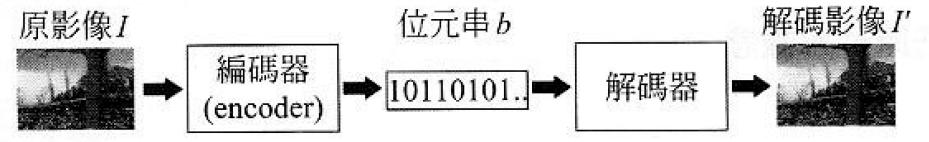
\includegraphics[scale=0.50]{figs/image_compression.jpg}
\label{f.imagecompressionbasics}
\end{figure}

Quando o sistema recebe a imagem original, ele manda para um codificador que converte a imagem original para um fluxo de bits. Um decodificador então recebe esse fluxo de bits e o transforma novamente na imagem. Caso o fluxo de bits final seja menor que o original, chamamos esse processo de Compressão de Imagem.

\citeauthor{mackenzielossless} diz que durante a compressão de uma imagem, pode-se ter perda de dados durante o processo. Por essa razão, o decodificador não consegue reconstruir a imagem perfeitamente para seu estado inicial. Esse tipo de compressão é chamado de Lossy, e esse processo é irreversível. O processo no qual a imagem pode retornar ao seu estado inicial é chamado de {\em Lossless}, o qual é possível reduzir o tamanho em disco, sem ter perda de dados durante o processo, sendo esse um processo reversível.

\section{Métodos de Compressão de Imagem Sem Perda}
\label{s.lossless}

São os chamados tipos de compressão {\em Lossless}. Neles, como dito anteriormente, é possível restaurar todos os dados originais da Imagem ao descompacta-la. Esse tipo de compressão é geralmente usado para arquivos de imagem de extensão GIF, formato usado na internet o qual são permitidas animação de imagens e utilização de transparência.

De acordo com \citeauthor{losslessmethods} define que compressão de imagens do tipo {\em Lossless}, também conhecidas como Compressão de Imagem Sem Perda, podem ser alcançadas através de Métodos de Codificação, Domínio Espacial, Domínio de Frequência, os quais são baseados em Transformadas, são uma combinação desses métodos.

Métodos de codificação são diretamente aplicados a imagens de formato RAW, o qual é o formato mais puro de uma imagem, normalmente sendo gerado a partir de câmeras profissionais. Esse formato acumula todos os dados necessários da imagem, como abertura da câmera, tipo da câmera, ISO utilizada, entre outras informações. O método de codificação trata a imagem como uma sequência de números discretos. Métodos comuns dessa incluem aritmética, Huffman, Lempel-Ziv Welch e Run-Length.

Métodos de domínio espacial são uma combinação de algoritmos de domínio espacial e métodos de codificação. Eles não somente operam diretamente nos tons de cinza, que são tons atribuidos a um pixel sendo 0 equivalente a branco e 100 equivalente a preto, como também tentam eliminar a redundância espacial. Essa redundância consiste na semelhança de pixels adjacentes de uma imagem. Suponhamos o seguinte exemplo: uma imagem de um avião passando no céu sem nuvens, na qual a informação relevante a ser transmitida é o avião, e o fundo é a parte da imagem azul cujo conteúdo da imagem é praticamente uniforme.

Na compressão de domínos de frequência, a imagem é representada usando uma base apropriada, com o objetivo de se obter um coeficiente de matriz pequeno. Transformada do Cosseno Discreto (DCT) e Transformada Wavelet são exemplos de compressão de domínio de frequência.

\subsection{Performance}
\label{ss.losslessperformance}

Perfomance em algoritmos do tipo {\em Lossless} pode ser especificados em termos de complexidade e eficiência.

A complexidade de um algoritmo de compressão de imagem é medida pelo número de operações aritméticas necessárias para realizar ambos processos de codificação e decodificação. Esse é um fator importante para aplicações que envolvem compressão online, onde a velocidade é crucial.

Eficiência de compressão é medida pela proporção de compressão ou pela taxa de bits. Proporção de compressão é o número de bits por pixel de uma imagem comprimida. Por exemplo, se uma imagem de dimensões 256x256 de 8 bits por pixel, é necessários 256 * 256 * 8 bits = 65.536 bytes quando armazenada em sua forma original. Se a imagem otimizada possuir 32.768 bytes, então a proporção de compressão será 65536 / 32768 = 2. Como a imagem possui dimensão de 256x256 = 65.536 pixels, o arquivo comprimido precisa de 32768 * 8 / 65536 = 4 bits, o qual será a taxa de bits necessária. A proporção de compressão portanto está associada a taxa de bits necessária. Sendo {\em CR} a proporção de compressão, {\em BR} a taxa de bits e {\em v} o número de bits por pixel de uma imagem não otimizada, temos a seguinte fórmula:

\[ CR = b / BR \]

\subsection{Métodos de Codificação}
\label{ss.codingmethod}

Nessa seção, serão abordados alguns algoritmos de codifição, bem como a explicação do método.

Para casos de codificação na qual uma imagem em duas dimensões será comprimida, existe a necessidade de convertê-la para uma sequência de uma dimensão. Para esse processo, chamamos de Linearização.

\subsubsection{Linearização}
\label{sss.linearlization}

A linearização não afeta a frequência da codificação, sendo esse método aplicado para alguns casos. Como Huffman depende somente da frequência dos diferentes tons de cinza, o método não é afetado pela linearização. Agora métodos como Liv-Zempel dependem da ordem dos tons de cinza, sendo então afetados por métodos de linearização.

Imagens possuem o que é chamado de redundância local, o que causa uma certa região da imagem a exibir uma coerência ou correlação, resultando em uma suavidade entre os pixels. Alguns métodos de linearização são mais efetivos que outros em se tratando de preservar essa região e, por isso, são esperados terem melhor desempenho quando combinadas com métodos de codificação que se utilizam dessas regiões de redundância.

Abaixo está uma lista dos métodos de linearização mais utilizados, segundo \citeauthor{losslessmethods}:

\begin{alineas}
    \item Verificação orientada por linha ({\em Row-Major Scan}): a imagem é verificada linha por linha, sentido cima-esquerda para baixo-direita;
    \item Verificação orientada por coluna ({\em Column-Major Scan}): a imagem é verificada coluna por coluna, com sentido cima-esquerda para baixo-direita;
    \item Verificação orientada por diagonal ({\em Diagonal Scan}): a imagem é verificada em diagonais, começando do canto inferior esquerdo para o canto superior direito;
    \item Verificação em formato de cobra ({\em Snake-like row-major Scan}): é uma variação da verificação orientada por linhas e orientada por colunas. Nela, ao chegar no final de uma linha, segue para a linha de baixo continuando na mesma coluna;
    \item Verificação em espiral ({\em Spiral Scan}): nesse método,;
    \item Verificação de Peano-Hilbert ({\em Peano-Hilbert Scan}): essa verificação requer que a imagem seja \[ 2^k * 2^k \]. Quando {\em k} é ímpar, o caminho percorrido começa no pixel mais a esquerda da primeira linha e termina no pixel mais a esquerda da última linha. Quando {\em k} é par, o caminho começa no pixel mais a esquerda da primeira linha e termina no pixel mais a direita da última linha.;
\end{alineas}

Segundo o autor, embora que nenhum método de linearização forneça a melhor compressão, a verificação de Peano-Hilbert geralmente traz o melhor resultado.

\subsubsection{Codificação de Huffman}
\label{sss.huffmancoding}

Nesse método, a redundância de codificação é eliminada com base numa codificação que produz um código de tamanho variável, atribuindo os códigos de tamanhos menores aos níveis de cinza mais prováveis de ocorrer.

Esse método possui duas etapas:

\begin{alineas}
    \item Cria-se uma série de reduções dos símbolos através da junção dos dois de menores probabilidades a cada iteração.
    \item Codificam-se todos os símbolos que foram reduzidos, começando com o de maior probabilidade que será associado ao menor código e voltando para os originais.
\end{alineas}

\citeauthor{losslesscodings} dá o seguinte exemplo: imagem de tamanho 10x10 e 6 tons de cinza (a1, a2, a3, a4, a5, a6), tendo as seguintes probabilidades de ocorrência: 5/8 de a1, 3/32 de a2 e a3, 1/32 de a6 e a4, e 1/8 de a5.

\begin{figure}[h]
\caption{\small Primeira etapa de codificação de Huggman.}
\centering
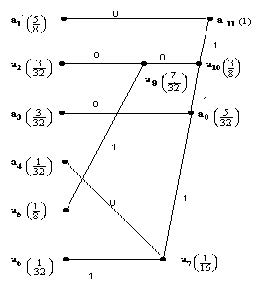
\includegraphics[scale=0.50]{figs/huffman_etapa1.jpg}
\label{f.huffmanetapa1}
\end{figure}

Tabela referente a segunda etapa da codificação de Huffman para as probabilidades das palavras mostradas na figura anterior.

\begin{table}[]
    \begin{center}
        \caption{\small Segunda etapa da codifiçãode Huggman}
        \label{t.huffmanetapa2}
        \begin{tabular}{llr}
            Informação & Probabilidade & Código \\
            a1         & 5/8 = 20/32   & 0      \\
            a10        & 3/8 = 12/32   & 1      \\
            a9         & 7/32          & 10     \\
            a8         & 5/32          & 11     \\
            a5         & 1/8 = 4/32    & 101    \\
            a2         & 3/32          & 100    \\
            a3         & 3/32          & 110    \\
            a7         & 2/32          & 111    \\
            a4         & 1/32          & 1110   \\
            a6         & 1/32          & 1111
        \end{tabular}
    \end{center}
\end{table}

Para transmitir essa informação, obtem-se uma taxa média de bits/informação seguindo a seguinte fórmula:

\[ (5/8)*1 + (3/32)*3 + (3/32)*3 + (4/32)*3 + (1/32)*4 + (1/32)*4 = 1,813 \]

\subsubsection{Codificação por LZW}
\label{sss.lzw}

Lempel, Ziv e Welch propuseram um método de codificação adaptável que não requer que todos que irão ser compressados, estejam disponíveis desde o começo. Essa técnica gera o código conforme o vai examinando, do começo ao fim. Na codificação por Huffman, um código de tamanho variável é construído para cada símbolo no código fonte. Na codificação Lampel-zev, códigos de tamanho fixo são construídos a medida que o processo vai rodando, para cada sequência de símbolos de tamanho variável.

Suponhamos que os símbolos que ocorrem em um código seja {\em a}, {\em b}, e {\em c}, e que a cadeia de caracteres {\em ababcabc} está para ser comprimida. Primeiro, iniciamos o dicionário para essa tradução no qual apenas um símbolo seja possível. Como o código do dicionário é dado pela posição, {\em a} seria 0, {\em b} seria 1 e {\em c} seria 2. Ao ler a cadeia de caracteres ababcabc, temos o primeiro sendo {\em a}. Seu código 0 seria parte do arquivo comprimido em conjunto com o prefixo e a próxima entrada. Nesse caso, seria {\em ab} e o código seria 3. A parte que restou para compressão agora seria {\em babcabc}. Novamente pegamos a cadeia de maior prefix que sobrou, sendo {\em b} nesse caso. Seu código é 1, somando com o próximo prefixo que é {\em a}, temos o código 4. Como agora temos no dicionário os caracteres {\em a} e {\em b}, a próxima sequência que pegaremos da cadeia restante, {\em abcabc} será {\em ab}. O código dela é 3, somando com o código do próximo caracter {\em c}, temos o valor 5. Como próxima sequência encontrada é {\em c}, com código 2 e temos {\em ca} entrando no dicionário. A cadeia restante então é {\em abc}, a qual está no dicionário, com valor 5. Com isso, foi possível chegar na codificação da cadeia {\em ababcabc}, a qual é 01325.

O método de compressão gzip, utilizado por sistemas Unix, utiliza uma combinação dos métodos de Huffman e LZW.

\subsubsection{Codificação por Código de Tons Corridos (RLE)}
\label{sss.runlength}

Nesse método, o código fonte é dividido em segmentos de símbolos idênticos. Cada segmento é separado por um símbolo e o número de ocorrências.

Para elucidar, suponha a cadeia {\em aaaabaaabb}. Ela é codificada como (a, 4), (b, 1), (a, 3), (b, 3). Esse método de codificação funcional bem para cadeias que possuem segmentos grandes, como imagens com fundos uniformes, porém esse método não é tão eficaz quando as cadeias possuem muitos segmentos curtos

\subsection{Métodos de Domínio Espacial}
\label{ss.transformmethod}

\citeauthor{pasteldeflango} diz que os algoritmos de domínio espacial envolvem métodos para reduzir o número de bits que representam a informação contida na imagem operando diretamente em seu formato mais cru, o qual contém maior número de informações. Tais métodos geralmente envolvem duas etapas. O primeiro estágio envolve o uso de técnicas como segmentação de imagem, amostras e interpolarização. Essa etapa é seguida por uma aproveita eficientemente as codificações produzidas pela primeira etapa.

Na primeira etapa, técnicas de segmentação de imagem incluem métodos de partição da imagem em formatos regulares, tais como retângulos, os quais ocupam menor armazenamento para codificar o formato devido a simplicidade, mas também podem assumir formatos irregulares, sendo esses últimos possuem um maior armazenamento devido a complexidade dos formatos resultantes do algoritmo de segmentação. Formatos mais simples necessitam de poucos bits para codificar a forma, mas possuem a restrição na representação, tendo um maior número de formas mais simples para representar a imagem total.

Muitos algoritmos dessa técnica são usadas nos métodos de compressão {\em Lossy}.

\subsubsection{Compressão de Tamanho de Bloco Variável}
\label{sss.variableblock}

\citeauthor{ranganathan} desenvolveu um algoritmo de compressão de imagens sem perda o qual explora redundâncias locais e globais da imagem. O algoritmo separa a imagem em blocos de tamanho variável e os codifica baseado nas propriedades que os pixels exibem no conjunto de cada bloco. Essa codificação é alcançada através do método de codificação por tons corridos (RLE) quando todos os pixels contidos no mesmo bloco possuem a mesma variação de tons de cinza, explorando assim a redundância local da imagem. Esse algoritmo explora a redundância global ao verificar se na região presente, existem blocos idênticos na região vizinha.

\subsubsection{Abordagem residual + Lossy}
\label{sss.lossyresidual}

O conceito desse método se dá de maneira que uma imagem já comprimida por métodos {\em Lossy}, de maneira que a imagem em si não seria possível ser reconstruída com todos os dados originais, é enviada seguida de resíduos da imagem original. Desse modo, é possível recontruí-la ao seu estado original.

Uma maneira de transmitir dados do tipo {\em Lossy} é através do resultado final de um algoritmo {\em Lossy}. Os resíduos da imagem original podem ser obtidos através de linearização, ou mesmo através de uma sequência de métodos efetivos de compressão, como Huffman citado anteriormente. Esse resíduo é basicamente a diferença da imagem original e a imagem reconstruída a partir da imagem comprimida.

A vantagem desse método é que utiliza de métodos {\em Lossy}, os quais possibilitam uma taxa alta de compressão.

Um exemplo desse método seria o conceito da compressão JPEG. Embora JPEG seja um tipo de compressão com perda, seu conceito foi capaz de basear algoritmos {\em Lossless}. O conceito especifica dois métodos de codificação para operações {\em lossless}:

\begin{alineas}
    \item Método de codificação de Huffman
    \item Método com codificação aritmética
\end{alineas}

Essa abordagem JPEG utiliza de técnicas de código preditivo e é totalmente independente de codificação utilizando transformadas, sendo que aplica codificação diferencial de forma a gerar os resíduos, sendo então codificados usando ou a técnica de Huffman ou codificação aritmética. Os resíduos são formado utilizando pixels previamente codificados na coluna atual ou então na coluna anterior. O residual {\em x} de um pixel é definido como sendo \[ R = Px - x \] onde {\em Px} é o valor previsto e pode ser qualquer valor definido na Tabela \ref{t.jpegstandart}, onde os valores {\em a}, {\em b} e {\em c} são pixels vizinhos ao pixel que está sendo analizado, como mostra Figura \ref{f.jpegstandart}.

\begin{table}[]
    \begin{center}
        \caption{\small Valores de predição para o método JPEG sem perda}
        \label{t.jpegstandart}
        \begin{tabular}{llr}
            Valor selecionado   & Equação de predição   \\
            0                   & sem predição          \\
            1                   & Px = a                \\
            2                   & Px = b                \\
            3                   & Px = c                \\
            4                   & Px = a + b - c        \\
            5                   & Px = a + (b - c)/2    \\
            6                   & Px = b + (a - c)/2    \\
            7                   & Px = (a + b)/2        \\
        \end{tabular}
    \end{center}
\end{table}

\begin{figure}[h]
\caption{\small Amostras utilizadas pela predição JPEG sem perda}
\centering
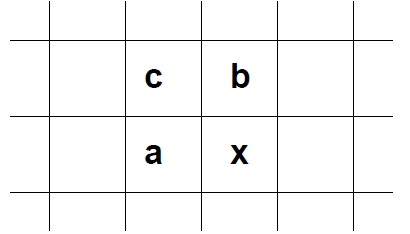
\includegraphics[scale=0.50]{figs/jpeg_standart.png}
\label{f.jpegstandart}
\end{figure}

\subsection{Métodos de Domínio de Frequência}
\label{ss.transformmethod}
